\hypertarget{group__EventGroupHandle__t}{}\section{Event\+Group\+Handle\+\_\+t}
\label{group__EventGroupHandle__t}\index{Event\+Group\+Handle\+\_\+t@{Event\+Group\+Handle\+\_\+t}}
Collaboration diagram for Event\+Group\+Handle\+\_\+t\+:\nopagebreak
\begin{figure}[H]
\begin{center}
\leavevmode
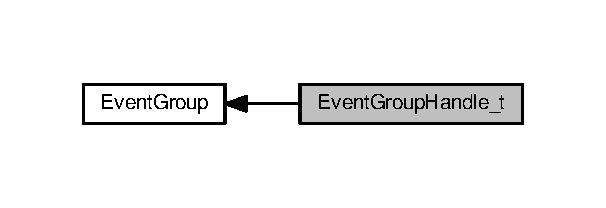
\includegraphics[width=291pt]{dc/d43/group__EventGroupHandle__t}
\end{center}
\end{figure}
\hyperlink{event__groups_8h}{event\+\_\+groups.\+h}

Type by which event groups are referenced. For example, a call to x\+Event\+Group\+Create() returns an Event\+Group\+Handle\+\_\+t variable that can then be used as a parameter to other event group functions. 